\documentclass{standalone}
\usepackage{tikz}
\usepackage{amsmath, amssymb}

\begin{document}

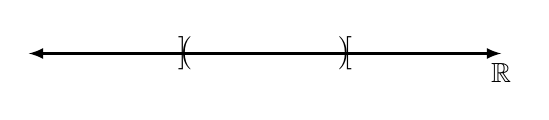
\begin{tikzpicture}
    % Draw the real number line
    \draw[thick, latex-latex] (-3, 0) -- (3, 0);
    \node[below] at (3, 0) {$\mathbb R$};

    % Mark points a and b on the number line
    % \node[below] at (-2, 0) {a};
    % \node[below] at (2, 0) {b};
    
    % Draw parentheses (open interval)
    \node at (-1.0, 0) {\large$($}; % arc[start angle=90, end angle=270, radius=0.15];
    \node at (1.0, 0) {\large$)$}; %arc[start angle=90, end angle=-90, radius=0.15];
    
    % Draw ] and [ just outside the parentheses
    \node at (-1.05, 0) {\large]};
    \node at (1.05, 0) {\large[};
    
\end{tikzpicture}

\end{document}
